\documentclass[11pt]{report}
\usepackage{ucs}
\usepackage[utf8x]{inputenc}
\usepackage[T1]{fontenc}
\usepackage[ngerman]{babel}
\usepackage{amsthm,amsmath,amssymb,amstext}
\usepackage{listings}
\usepackage{color}  
\usepackage[svgnames]{xcolor} 
\usepackage{ulem}
\usepackage{graphicx}
\usepackage{stmaryrd}
\usepackage{pdfpages}
\usepackage{paralist}
\usepackage{ae}
\usepackage{anysize}
\usepackage{lmodern,dsfont}
\usepackage[]{hyperref}
\hypersetup{%
  colorlinks= true,  
  linkcolor = black,  
  citecolor = black,
  urlcolor = black,  
} 

\marginsize{35mm}{30mm}{20mm}{20mm}

\title{\textbf{SQL-Alchemist-Teamprojekt} \\ API-Dokumentation}
\author{Tobias Grünhagen, Philip Holzhüter, Tobias Runge}
\date{\today}

\begin{document}

\maketitle

\chapter{Allgemeines}

Die API für das SQL-Alchemist-Projekt des IFIS an der Technischen Universität Braunschweig im Sommersemester 2015 dient dazu wichtige Grundfunktionen, wie das Verwalten von Aufgaben und der Datenbankanfragen, für das SQL-Lernspiel bereitzustellen.

Zuerst wird ein XML-File eingelesen, in dem die einzelnen Aufgaben bereitgestellt werden. Dabei wird die Struktur validiert und bereits der Aufbau der SQL-Statements gecheckt. Beim Parsen des Dokuments wird für jede Aufgabe ein neuer Task angelegt, über den die komplette Aufgabe verwaltet werden kann. Die für die Aufgabe nötigen Tabellen und Einträge werden in einer aufgabenspezifische Datenbank abgespeichert, die wieder gelöscht wird, falls sie nicht mehr benötigt wird. Anfragen an die Datenbank und auch der Zugriff auf einzelne Komponenten der Aufgabenstellung kann komplett über den Task verwaltet werden.

Die Programmstruktur und die Programmzusammenhänge können in dem folgenden Klassendiagramm nachvollzogen werden. Bei Benutzung der API sollte ein InputFile-Objekt mit dem Namen des XML-Files erstellt werden. Hier wird im Konstruktor automatisch die Struktur durch die XMLSyntaxCheck-Klasse validiert und mit Hilfe der MySAXParser-Klasse das Dokument eingelesen. Im MySAXParser werden nach dem Parsen mit Hilfe der DBConnection-Klasse die einzelnen SQL-Statements gecheckt. Dann wird für jede Aufgabe ein neues Task-Objekt erstellt, in welchem jeweils ein Header-Objekt, ein Exercise-Objekt und Relation-Objekt gespeichert werden. In jedem Task wird beim starten der Aufgabe in einer festen Datenbank überprüft, ob der Task bereits gespielt wird. Ist dem so, wird für die Aufgabe die bereits bestehende aufgabenspezifische Datenbank benutzt, ansonsten wird eine neue Datenbank angelegt. Hierbei werden die CREATE-TABLE- und INSERT-Statements aus der Aufgabenstellung mit Hilfe von Exercise- und Relation-Objekten ausgeführt. Spielt am Ende der Bearbeitung einer Aufgabe kein Spieler mehr die Aufgabe, wird die aufgabenspezifische Datenbank gelöscht. So wird der Verbleib von Datenmüll und Datenleichen vermieden. In einem Task können während des Spielens SQL-Anfragen an die Datenbank gestellt werden, hierfür wird die DBConnection-Klasse verwendet.

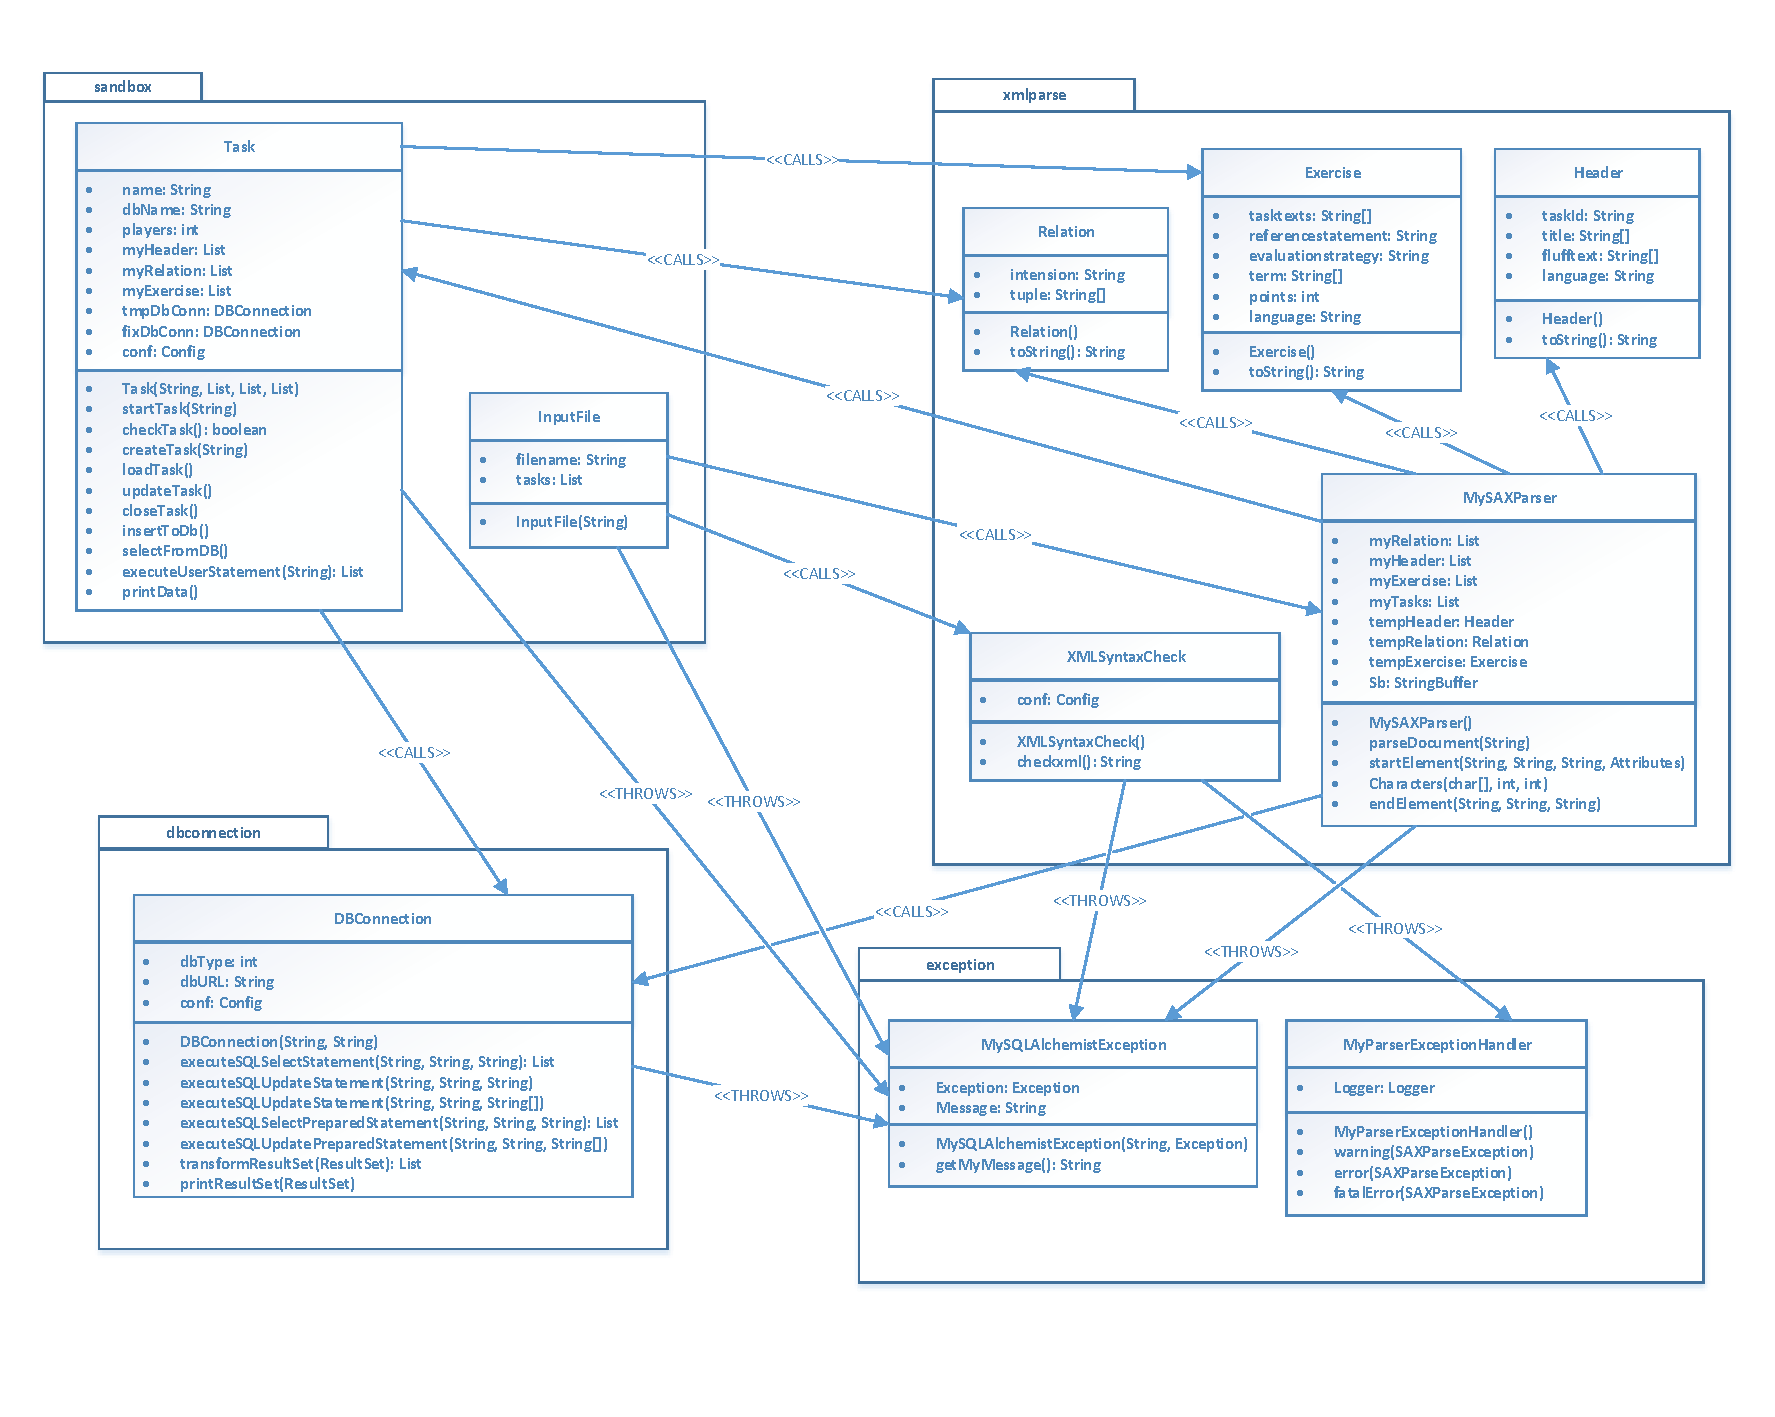
\includepdf{Klassendiagramm.pdf}

\chapter{Klassenerläuterungen}

Im Folgenden werden die Funktionen der einzelnen Klassen erläutert.

\section{InputFile.java}

Diese Datei ist der Startpunkt, wenn man eine neue XML-Datei einlesen und einen neuen Task starten möchte. Der Konstruktor möchte als Parameter eine XML-Datei ohne die Endung \grqq .xml\grqq. Diese Datei wird ihre auf Syntax geprüft, geparst und für jeden Task innerhalb dieser Datei wird ein Task-Objekt erzeugt.

\subsection*{Klassenvariablen}

String \textit{filename}: Name der XML-Datei ohne die Dateiendung \grqq .xml\grqq\  \\
List \textit{tasks}: Liste aller Tasks, die im Konstruktor erzeugt werden

\subsection*{Konstruktor}

Parameter: XML-Datei ohne die Dateiendung \grqq .xml\grqq\ \\
Checkt und parst die Datei, dabei werden Fehler geworfen, falls die Datei nicht korrekt ist.
Falls alles korrekt ist, wird für jeden Task in der Datei ein Task-Objekt erzeugt und in die Liste \textit{tasks} gespeichert.

\section{Exercise.java}

Hier finden sich alle Inhalte aus der XML-Datei, die unter \textit{subtasks} zu finden sind. In jedem Objekt ist immer ein Subtask gespeichert.

\subsection*{Klassenvariablen}

String[] \textit{tasktexts}: Die Aufgabenstellung der Aufgabe in Deutsch und Englisch, falls vorhanden \\
String \textit{referencestatement}: Das Lösungsstatement der Aufgabe \\
String \textit{evaluationstrategy}: Rückgabetyp der Aufgabe (Liste oder Menge) \\
String \textit{term}: Die Terme, die für die Lösung der Aufgabe benötigt werden \\
int \textit{points}: Die Punkte für die Aufgabe bzw. der Schwierigkeitsgrad \\
String \textit{language}: Die Sprache für die Aufgabe (wird beim Parsen nicht gesetzt)

\section{Header.java}

Hier finden sich alle Inhalte aus der XML-Datei, die am Anfang jedes Tasks stehen.

\subsection*{Klassenvariablen}

String \textit{taskId}: Die eindeutige ID der Aufgabe \\
String[] \textit{title}: Die Überschrift der Aufgabe \\
String[] \textit{flufftext}: Die allgemeine Beschreibung der Aufgabe \\
String \textit{language}: Die Sprache für die Aufgabe (wird beim Parsen nicht gesetzt)

\section{Relation.java}

Hier finden sich alle Inhalte aus der XML-Datei die unter \textit{schema} zu finden sind. In jedem Objekt ist immer eine Relation gespeichert.

\subsection*{Klassenvariablen}
String \textit{intension}: Ein Create-Table-Statement der Aufgabe \\
String[] \textit{tuple}: Die zugehörigen Insert-Into-Statements der Aufgabe

\section{Task.java}

Diese Klasse enthält alle Methoden zum Verwalten von Tasks. Die Klassenvariablen sind zum einen Listen für sämtliche Inhalte des XML-Dokuments und zum Anderen die benötigten Datenbankverbindungen, für die Spielübersicht und für die einzelnen Tasks.

\subsection*{Klassenvariablen}
String \textit{name}: Name des Tasks \\
String \textit{dbName}: Name der zum Task gehörenden Datenbank \\
int \textit{players}: Anzahl der Spieler dieses Tasks \\
List \textit{myHeader}: Liste der Header einer XML-Datei \\
List \textit{myRelation}: Liste der Inhalte des XML-Dokuments im Bereich \textit{schema}. \\
List \textit{myExercise}: Liste der Subtasks eines XML-Dokuments \\
DBConnection \textit{tmpDbConn}: Datenbankverbindung zur zum Task gehörenden Datenbank \\
DBConnection \textit{fixDbConn}: Datenbankverbindung zur Datenbank für die Spielübersicht

\subsection*{Methoden}

\subsubsection*{startTask(String dbType)}	

Die Methode \textit{startTask} dient im Allgemeinen dazu, einen neuen Task zu starten, bzw. ihn zu laden, falls so ein Task noch nicht existiert.

Der Parameter \textit{dbType} gibt den Datenbanktyp an. Dabei kann es sich entweder um eine lokale Datenbank, eine InMemory-Datenbank oder eine Online-Datenbank handeln.

Zunächst wird die Methode \textit{checkTask()} aufgerufen. Wenn so ein Task noch nicht besteht, die Methode also den Wert \textit{false} liefert, wird die Spielerzahl dieses Tasks auf den Wert 1 gesetzt und die Methode \textit{createTask()} aufgerufen. Falls jedoch bereits ein solcher Task besteht, so wird dieser Task aus der Datenbank zur Spielübersicht geladen, die Spielerzahl um den Wert 1 erhöht, das XML-Dokument auf Syntaxfehler geprüft und dann schließlich geparst. Anschließend wird noch der Task aktualisiert indem \textit{updateTask()} aufgerufen wird.
	
\subsubsection*{checkTask()}

Die Methode \textit{checkTask} soll prüfen ob der Task bereits existiert.

Dazu wird auf der Datenbank zur Spielübersicht ein Prepared-Statement ausgeführt, welches alle Tasks mit dem aktuellen Namen liefert (entweder liefert es einen Eintrag oder eine leere Tabelle). Dadurch kann ein boolean-Wert zurückgegeben werden, ob der Task bereits existiert oder nicht.


\subsubsection*{createTask(String dbType)}

Die Methode \textit{createTask} erstellt im Allgemeinen einen neuen Task. 

Der Parameter \textit{dbType} gibt den Datenbanktyp an (s. \textit{startTask}).
Zunächst wird in der Datenbank zur Spielübersicht ein neuer Eintrag für diesen Task angelegt. Danach wird eine Datenbank für diesen Task angelegt, auf der nach dem XML-Syntax-Check und dem Parsen des Dokuments alle Statements ausgeführt werden können (alle dafür notwendigen  Tabellen werden erstellt etc.)

\subsubsection*{loadTask()}

Die Methode \textit{loadTask} lädt mittels Prepared-Statement einen bereits existierenden Task und eine Datenbank, auf der später alle Statements ausgeführt werden können.

\subsubsection*{updateTask()}

Die Methode \textit{updateTask} aktualisiert in der Datenbank zur Spielübersicht den Eintrag zum aktuellen Task (erhöhen bzw. erniedrigen der Spielerzahl).

\subsubsection*{closeTask()}

Die Methode \textit{closeTask} löscht einen Task und verringert dabei die aktuelle Spielerzahl um den Wert 1. Falls der aktuelle Task keine Spieler mehr hat, die Spielerzahl also den Wert 0 hat, wird die zum Task gehörige Datenbank mit all ihren Inhalten des Aufgabenblattes gelöscht.

\subsubsection*{insertToDb()}

Die Methode \textit{insertToDb} lädt alle Inhalte der Aufgabenblätter in die zugehörige Datenbank. 
Dabei wird über die Liste der Relationen iteriert und jedes Element dann über ein Prepared-Statement in die Datenbank geladen.

\subsubsection*{selectFromDb()}

Die Methode \textit{selectFromDb} führt alle Reference-Statements des Aufgabenblattes aus, liefert dabei aber nicht die Ergebnisse dieser Statements zurück, sie dient primär dazu die Reference-Statements auf Ausführbarkeit zu prüfen.
Dabei wird über die Liste der Exercises iteriert und jedes Element dann über ein Prepared-Statement auf der Datenbank ausgeführt.

\subsubsection*{executeUserStatement(String statement)}

Die Methode \textit{executeUserStatement} dient dazu ein User-Statement auszuführen und die Ergebnisse dieses Statements zurückzuliefern.
Dabei wird das Statement (String) als Parameter an die Methode übergeben und dann auf der Datenbank ausgeführt. Das Ergebnis der Abfrage wird dann zurückgeliefert.

\subsubsection*{printData()}

Die Methode \textit{printData} gibt alle Inhalte des Aufgabenblattes aus.
Es wird für jede der drei Listen nacheinander (für die Header, Relations und Exercises) die Anzahl der Elemente und anschließend die Elemente selbst ausgegeben.

\chapter{Datengenerierung}

\section{XML-Tags}

Wir benötigen zusätzliche Informationen in der XML-Datei, damit wir Daten generieren können. Ein Beispiel zeigen wir in \autoref{code:xml}. Innerhalb des \texttt{relation-Tags} benötigen wir ein \texttt{metadata-Tag}. In diesem wird im Tag \texttt{tablename} der Name der Tabelle, wie in der intension angegeben, genannt. Außerdem benötigen wir pro Primärschlüssel den Tag \texttt{primarykey} in dem der Schlüssel angegeben wird. Zum Schluss folgt der Tag \texttt{datageneration} mit dem die Daten generiert werden können. Dieser Tag kann mehrmals benutzt werden, sollte mehrere verschiedene Daten der Tabelle hinzugefügt werden. Der genaue Aufbau für die Datengenerierung folgt in \autoref{cha:aufbau}.

\begin{figure}[h]
	\centering
	\begin{minipage}{0.9\textwidth}
		\lstinputlisting[
			caption={XML-Datei für die Meta-informationen},
			label={code:xml}
		]{Beispiel.xml}
	\end{minipage}
\end{figure}


\section{Aufbau für die Datengenerierung}
\label{cha:aufbau}

Im Folgenden wird erläutert wie Daten generiert werden können. Der Allgemeine Aufbau ist:

\texttt{Anzahl;Ref;Spalte1;Spalte2;Spalte3;...}

\bigskip\noindent
Anzahl besteht aus einer Zahl oder \texttt{span,Anfang,Ende}\\
Ref ist noch nicht implementiert und im Moment sollte \texttt{none} angegeben werden\\
Spalte: hier werden die Daten für eine Spalte generiert und alle Parameter werden durch ein Komma getrennt. Also ist der Aufbau einer Spalte:

\texttt{Para1,Para2,Para3,...}

\bigskip\noindent
\textbf{erste Parameter:}
\begin{itemize}

\item random: zufälliger Eintrag
\begin{itemize}
\item	int, int+, double, string(optional mit Länge), firstname, lastname, fullname, date, business, street, adress, email, custom(name, opt. random, opt. Default)
\begin{itemize}
\item	für den Parameter name nach custom gibts folgende Möglichkeiten: alias, chemical element, colour, comic title, effect, gender, genre, land, occupation, programming language, publisher, size
\end{itemize}
\end{itemize}

die Angaben in Klammern sind weitere Parameter
Beispiel: random,string,5 oder random,firstname oder random,colour,80,weiß

\item min: mindestens größer als
\begin{itemize}
\item int(min), double(min)
\end{itemize}

\item max: maximal so groß
\begin{itemize}
\item int(max), double(max)
\end{itemize}

\item between: zwischen zwei Werten
\begin{itemize}
\item int(min, max), double(min, max)
\end{itemize}
	

\item gauss: gaussche Normalverteilung
\begin{itemize}
\item int(Mittelwert, Standardabweichung), double(Mittelwert, Standardabweichung)
\end{itemize}


\item list: liste von Zahlen mit Parameter Start

\item fix: selbst ausgedachter Wert: Wert mit '' also fix,'ausgedacht'
\end{itemize}

weitere Beispiele: min,int,5 oder gauss,int,5,4

\bigskip\noindent
Sollen für eine Tabelle Daten generiert werden, die eine andere Tabelle referenziert, muss bei der entsprechenden Spalte angegeben werden, auf welche Spalte einer anderen Tabelle sich diese Spalte bezieht. Wie in \autoref{code:xml2} ersichtlich wird für die Spalte \texttt{ref,Tabellenname,Spalte} angegeben, also z.B. \texttt{ref,powders,id}.

\begin{figure}[h]
	\centering
	\begin{minipage}{0.9\textwidth}
		\lstinputlisting[
			caption={weitere XML-Datei für die Meta-informationen},
			label={code:xml2}
		]{Beispiel2.xml}
	\end{minipage}
\end{figure}

\end{document}
